\chapter{Przegląd literatury}
\label{cha:literatura}

Problem skutecznej detekcji oraz unikania przeszkód przez roboty mobilne lub drony często pojawia się w projektach z dziedziny robotyki opisanych w literaturze. Potrzeba integracji takich systemów wynika z chęci zwiększenia ich autonomiczności -- każdy system sterowania robotem mobilnym, który ma działać samodzielnie, bez ingerencji operatora, musi być wyposażony w system pełniący taką funkcję.

Do detekcji zagrożeń na trasie robota często wykorzystuje się proste czujniki zbliżeniowe lub czujniki odległości. W ten sposób jednak uzyskuje się jedynie stosunkowo późną informację o obecności lub dodatkowo o odległości do przeszkody. Takie podejście okaże się wystarczające, jeśli robot porusza się wolno, przeszkody są duże i nieruchome, a wymagana reakcja robota na wystąpienie barier na trasie nie wymaga żadnych dodatkowych danych (przykładowo -- robot skręca w prawo o 90 stopni, za każdym razem gdy napotka przeszkodę).

Realizowany w ramach projektu system powinien jednak mieć szersze możliwości. Oprócz dostarczania danych o wystąpieniu przeszkody, ma on za zadanie informować także o jej położeniu, kształcie oraz prędkości, a wszystko to odpowiednio wcześnie, tak aby możliwe było zaplanowanie trajektorii i zapewniona możliwość szybkiego przemieszczania się robota. Takie podejście do problemu daje możliwości reakcji na przeszkody będące w ruchu oraz na realizację bardziej złożonych algorytmów sterowania w celu ich skutecznego uniknięcia.

% Ta część może pójdzie do terii potem
Sposoby wykrywania przeszkód zebrane i~opisane są w~artykułach \cite{detection_techniques}, \cite{detection_methods} oraz w~\cite{detection_methods2}. Detekcja obiektów może być realizowana na podstawie danych pochodzących z~różnych typów czujników. Najczęściej wykorzystywane sensory to:
\begin{itemize}
    \item LiDAR (ang. \textit{Light Detection and Ranging}) -- czujnik zbierający przestrzenne dane o~otoczeniu (odległości do otaczających go obiektów), za pomocą krótkich sygnałów świetlnych. Główną zaletą jest wysoka precyzja, natomiast wadą -- duża ilość danych, które należy przetworzyć, a~więc wysokie wymagania obliczeniowe systemów opartych na tych czujnikach.
    \item RADAR (ang. \textit{Radio Detection and Ranging}) -- działa dzięki sygnałom radiowym. Charakteryzuje się potencjalnie dużym dystansem detekcji, ale może mieć problem z~wykrywaniem obiektów niewielkich oraz takich, które słabo odbijają fale w~tym zakresie.
    \item SONAR (ang. \textit{Sound Navigation and Ranging}) -- wykorzystuje sygnały dźwiękowe i~używany jest głównie tam, gdzie warunki negatywnie wpływają na działanie innych czujników (np. pod wodą).
    \item Czujniki ultradźwiękowe -- to urządzenia wykorzystujące fale dźwiękowe o~wysokiej częstotliwości (powyżej zakresu słyszalnego dla ludzkiego ucha, tj. > \SI{20}{kHz}) do wykrywania obiektów i~mierzenia odległości. Działają na zasadzie emisji ultradźwięków i~analizy echa odbitego od przeszkody. Ich zaletą jest niezależność od oświetlenia sceny i~niski koszt, natomiast wadą stosunkowo niewielki dystans detekcji.
    \item Kamery -- niewątpliwą zaletą ich stosowania jest niska cena. % w porównaniu do czujników aktywnych (czyli posiadających własne źródło energii -- wszystkie powyższe).
    Wykorzystując kamery do detekcji obiektów, stosuje się różne podejścia. Przeszkody można wykrywać na podstawie ich znanych właściwości -- kształtu i~rozmiaru, lub na podstawie ich ruchu i~prędkości. Projektuje się systemy wykorzystujące pojedynczą kamerę, jak i~takie z dwiema kamerami skonfigurowanymi w~układ stereo, co daje większe możliwości przy obliczaniu głębi.
   %\item Czujniki ultradźwiękowe to urządzenia wykorzystujące fale dźwiękowe o~wysokiej częstotliwości (powyżej zakresu słyszalnego dla ludzkiego ucha, tj. >\SI{20}{kHz}) do wykrywania obiektów i~mierzenia odległości. Działają na zasadzie emisji ultradźwięków i~analizy echa odbitego od przeszkody. Ich zaletą jest niezależność od oświetlenia sceny i~niski koszt, natomiast wadą stosunkow niewielki dystans detekcji.
    \item \textbf{Kamery zdarzeniowe} -- szerzej opisane w~podrozdziale \ref{sec:kamery_zdarzeniowe}
\end{itemize}

% \section{Powiązane publikacje}
% \label{sec:przeglad}

W~literaturze znaleźć można artykuły opisujące projekty o~podobnej tematyce, w~ramach których został zaprojektowany i~zaimplementowany system detekcji i~unikania przeszkód. W~celu wyboru metody rozwiązania tego problemu przeanalizowano sposoby detekcji zastosowane w~wybranych, najbardziej zbliżonych do tematu projektu publikacjach. Cele w~tych artykułach częściowo pokrywają się z~celami projektu (\ref{sec:celePracy}), co pozwala na wzorowanie się na nich i~czyni je szczególnie pomocnymi~w realizacji zadania. 

\textbf{Dynamic obstacle avoidance for quadrotors with event cameras} (\textit{Davide Falanga, Kevin Kleber, Davide Scaramuzza}) \cite{dynamic_obstacle} -- projekt, w~którym autorzy zaprojektowali i~zaimplementowali system unikania przeszkód dla czterowirnikowego drona. Celem było ominięcie szybko poruszających się (do \SI{10}{\frac{m}{s}}) w~kierunku drona obiektów (na przykład rzuconej w~niego piłki -- rys. \ref{fig:dynamic_obstacle}). Statyczne bariery na trasie drona są ignorowane. System działa zarówno na zewnątrz, jak i~we wnętrzach budynków. Autorzy, oprócz skuteczności, skupiają się na osiągnięciu możliwie niskiej latencji w~wykrywaniu przeszkód -- końcowa wartość to $3.5$ $ms$. Jest to możliwe właśnie dzięki zastosowaniu kamer zdarzeniowych.

\begin{figure}
    \centering
    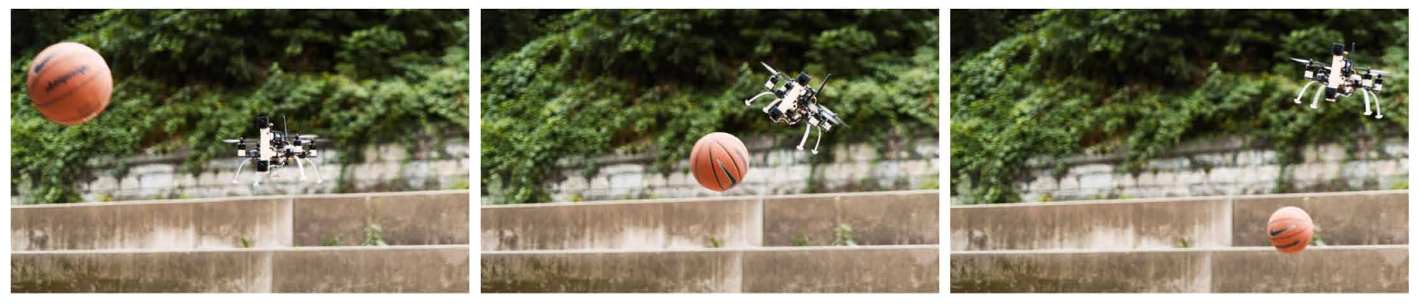
\includegraphics[width=0.8\linewidth]{images/dyanimc_obstacle.png}
    \caption{Przykład manewru uniku z projektu \cite{dynamic_obstacle}.}
    \label{fig:dynamic_obstacle}
\end{figure}

Na system detekcji przeszkód z~projektu \cite{dynamic_obstacle} składają się kolejne etapy:
\begin{enumerate}
    \item Kompensacja ruchu własnego drona -- autorom zależy na wykrywaniu wyłącznie poruszających się przeszkód, jednak zdarzenia w DVS generowane są również przez ruch  samego drona i~obiekty statyczne. Na podstawie danych z czujnika IMU (ang. \textit{inertial measurement unit}) -- rotacji drona, odróżniane są statyczne elementy sceny od dynamicznych.
    \item Segmentacja przeszkód -- dzięki wynikom poprzedniego etapu możliwe jest oddzielenie zdarzeń odpowiadających za przeszkody od statycznej części sceny. Dalej przetwarzane są tylko obiekty w~ruchu.
    \item Obliczenie przepływu optycznego za pomocą algorytmu Lucasa-Kanade \cite{Lucas-Kanade}, w~celu usprawnienia późniejszej klasteryzacji zdarzeń. Przepływ optyczny dostarcza dane o wektorach ruchu pikseli na obrazie, co ułatwia odróżnienie różnych obiektów, które znajdują się blisko siebie, ale poruszają się inaczej.
    \item Klasteryzacja -- za pomocą algorytmu DBScan \cite{DBScan} separuje się zdarzenia odpowiadające poszczególnym obiektom -- scena może zawierać wiele przeszkód. Dodatkową rolą tego etapu jest usunięcie szumu.
    \item Estymacja pozycji w przestrzeni 3D -- w~przypadku gdy używana jest tylko jedna kamera zdarzeniowa, autorzy w celu wyznaczenia głębi, ograniczają się do przeszkód o~znanym rozmiarze. Wtedy ich odległość od kamery może być łatwo wyznaczona na podstawie ich szerokości w~klatce obrazu.
    W~przypadku dwóch kamer w układzie stereo \cite{detection_methods}, możliwa jest estymacja głębi dla wszystkich obiektów za pomocą triangulacji \cite{view_geometry}.
    \item Projekcja pozycji przeszkód z układu współrzędnych kamery na układ współrzędnych świata i~estymacja prędkości przeszkód.

\end{enumerate}

\textbf{EVDodgeNet: Deep Dynamic Obstacle Dodging with Event Cameras} (\textit{Nitin J. Sanket, Chethan M. Parameshwara, Chahat Deep Singh, Ashwin V. Kuruttukulam,
Cornelia Fermüller, Davide Scaramuzza, Yiannis Aloimonos}) \cite{EVDodge} -- projekt, w którym problem zdefiniowany jest bardzo podobnie do \cite{dynamic_obstacle} -- unikanie przez drona szybko poruszających się obiektów różnych kształtów i~rozmiarów. Podejście do implementacji znacznie się jednak różni. Autorzy do kolejnych etapów detekcji obiektów na podstawie danych z~kamery zdarzeniowej wykorzystują szereg płytkich sieci neuronowych. Pierwsza z~nich odpowiedzialna jest za poprawę jakości ramek zdarzeniowych (usunięcie rozmycia, redukcja szumów). Kolejna odpowiada za uzyskiwanie odometrii (estymacja pozycji). Zadaniem ostatniej jest segmentacja niezależnie poruszających się obiektów. Modele trenowane były wyłącznie przy wykorzystaniu symulacji komputerowej. Skuteczność gotowego systemu autorzy oceniają na $70\%$. System przetestowany został również w~trudnych warunkach oświetleniowych, w~których mógł efektywnie pracować, dzięki zastosowaniu DVS. 

\textbf{Night vision obstacle detection and avoidance based on Bio-Inspired Vision Sensors} (\textit{Jawad Naveed Yasin,
                  Sherif Abdelmonem Sayed Mohamed,
                  Mohammad Hashem Haghbayan,
                  Jukka Heikkonen,
                  Hannu Tenhunen,
                  Muhammad Mehboob Yasin,
                  Juha Plosila}) \cite{night_obstacle} -
    projekt, w którym autorzy koncentrują się na detekcji przeszkód w ograniczonych warunkach oświetleniowych -- stąd wybór kamery zdarzeniowej. Zadanie to jest realizowane przy wykorzystaniu tradycyjnego podejścia -- bez głębokich sieci neuronowych. Działanie gotowego systemu zostało przetestowane na gotowych zbiorach danych. Na koniec porównane zostały wyniki otrzymane dla tradycyjnej kamery oraz DVS.

\begin{figure}
    \centering
    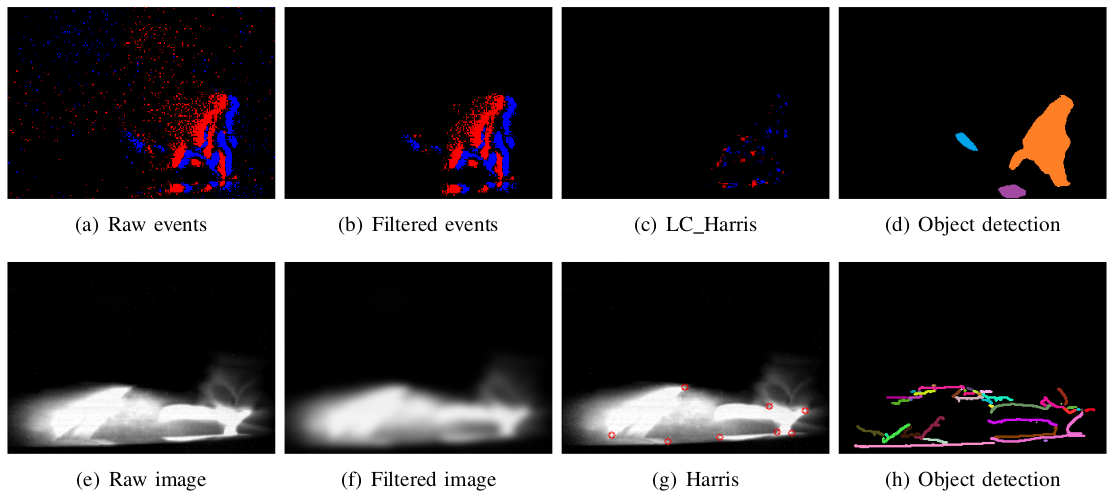
\includegraphics[width=0.8\linewidth]{images/night_obstacle.png}
    \caption{Porównanie działania algorytmu detekcji przeszkód z artykułu \cite{night_obstacle} dla DVS i~tradycyjnej kamery. Zastosowanie kamery zdarzeniowej umożliwia detekcję w nocnych warunkach.}
    \label{fig:night_obstacle}
\end{figure}

System detekcji przeszkód z projektu \cite{night_obstacle} działa w następujący sposób:
\begin{enumerate}
    \item Filtracja szumu tła -- w danych otrzymywanych z~kamery zdarzeniowej występują błędnie wygenerowane zdarzenia, które nie są częścią właściwego sygnału i~które należy z~niego usunąć w~celu obniżenia wymagań obliczeniowych dla późniejszych etapów (mniej zdarzeń do przetworzenia) oraz zwiększenia niezawodności algorytmu. W tym celu użyto algorytmu kNN (ang. \textit{k-nearest neighbour}) \cite{dba_filter}.
    \item Podział odczytywanych zdarzeń na grupy, jako które będą dalej przetwarzane. Do każdej \textit{klatki}, zapisywane jest $N$ zdarzeń. Wartość $N$ dobierana jest dynamicznie w~zależności od prędkości obiektów.
    \textit Dopasowanie płaszczyzn w~chmurze punktów -- zdarzeń, do poszczególnych obiektów na~scenie za pomocą algorytmu RHT (ang. \textit{Randomised Hough Transform}).
    \item Wyznaczenie punktów charakterystycznych za pomocą metody bazującej na algorytmie Harris \cite{Harris}. 
    \item Estymacja głębi dla każdej z przeszkód. Autorzy mimo zastosowania pojedynczej kamery, obliczają odległość za pomocą triangulacji, dzięki danym o pozycji i rotacji kamery.
\end{enumerate}

\begin{figure}
    \centering
    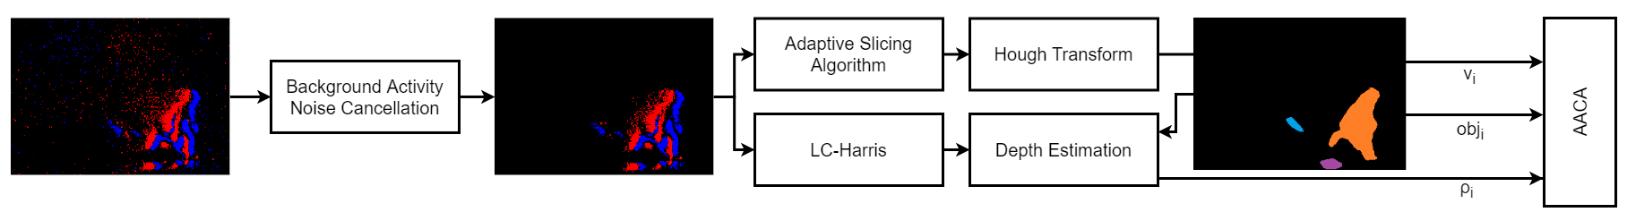
\includegraphics[width=1\linewidth]{images/overview_night_obstacle.png}
    \caption{Schemat działania algorytmu detekcji z~projektu \cite{night_obstacle}.}
    \label{fig:night_overview}
\end{figure}
    
%TODO tu by się przydało wymienić (choćby po 1 zdaniu) jeszcze kilka artykułów, może tych, które są wymienione poniżej: RED, ASTMNet itd.


% \section{Detekcja obiektów}

% Wykrywanie obiektów za pomocą danych z kamer zdarzeniowych







Innym, często spotykanym podejściem do wykrywania obiektów za pomocą kamer zdarzeniowych, jest użycie uczenia maszynowego i~głębokich sieci neuronowych. Tego typu modele do detekcji zostały stworzone w~ramach wielu dostępnych w~literaturze projektów i~stanowią bogatą bazę narzędzi. Przykładowo wymienić można algorytmy:
\begin{itemize}
    \item \textit{RED} \cite{RED} -- wprowadza rekurencyjną architekturę, umożliwiającą uczenie na podstawie zdarzeń bez konieczności rekonstrukcji obrazu,
    \item \textit{ASTMNet} \cite{ASTMNet} -- wykorzystuje moduł pamięci do detekcji obiektów w~sposób ciągły, eliminując potrzebę przekształcania zdarzeń na obrazy,
    \item \textit{RVT} \cite{RVT} -- redukuje czas przetwarzania do \SI{12}{\micro\s} przy zachowaniu wysokiej wydajności i~efektywności parametrów,
    \item \textit{DMANet} \cite{DMANet} -- wykorzystuje podwójną pamięć (modeluje ją jako krótko i długotrwałą) do skutecznej agregacji zdarzeń dla lepszej detekcji obiektów,
    \item \textit{TEDNet} \cite{TEDNet} -- wprowadza etykiety widoczności obiektów i~strategie ich śledzenia, umożliwiając detekcję w~przypadku braku relatywnego ruchu wobec kamery.
\end{itemize}

% \section{Inne wykorzystane projekty} % Może raczej wykorzystywane projekty, też: Śledzenie obiektów SORT 

% O v2e, ESim, SORT

% W literaturze można znaleźć wiele artykułów opisujących projekty, których autorzy stworzyli gotowe i~wygodne do wykorzystania w kodzie narzędzia, spełniające różne zadania, których realizacja w ramach tego projektu była wymagana. Użycie takich narzędzi ułatwia pracę oraz pozytywnie wpływa na efekt końcowy.

% \vspace{11px}
% \noindent \textbf{Symulacja DVS na podstawie klatek z tradycyjnej kamery}
% \vspace{11px}



% \vspace{11px}
% \noindent \textbf{Śledzenie obiektów}
% \vspace{11px}

% Problem śledzenia obiektów polega na przypisywaniu do nich indywidualnych identyfikatorów, tak aby możliwe było ich jednoznaczne rozpoznanie w kolejnych iteracjach algorytmu.
% W projekcie wykorzystywane jest do tego celu narzędzie SORT (ang. \textit{Simple Online and Real-time Tracking}) \cite{sort}, którego zaletą jest łatwość użycia w skryptach w języku Python.









